\documentclass{article}
\usepackage{listings}
\usepackage{mathrsfs}
\usepackage[utf8]{inputenc}
\usepackage{amssymb}
\usepackage{lipsum}
\usepackage{amsmath}
\usepackage{fancyhdr}
\usepackage{geometry}
\usepackage{scrextend}
\usepackage[english,german]{babel}
\usepackage{titling}
\setlength{\droptitle}{-3cm}
\usepackage{tikz}
\usepackage{algorithm,algpseudocode}
\usepackage[doublespacing]{setspace}
\usetikzlibrary{datavisualization}
\usetikzlibrary{datavisualization.formats.functions}
\usepackage{polynom}
\usepackage{amsmath}
\usepackage{verbatim}
\usepackage{gauss}
\usepackage{tkz-euclide}
\usetikzlibrary{datavisualization}
\usetikzlibrary{datavisualization.formats.functions}
\author{
Alexander Mattick Kennung: qi69dube\\
Kapitel 1
}
\usepackage{import}
\date{\today}
\geometry{a4paper, margin=2cm}
\usepackage{stackengine}
\parskip 1em
\newcommand\stackequal[2]{%
  \mathrel{\stackunder[2pt]{\stackon[4pt]{=}{$\scriptscriptstyle#1$}}{%
  $\scriptscriptstyle#2$}}
 }
\makeatletter
\renewcommand*\env@matrix[1][*\c@MaxMatrixCols c]{%
  \hskip -\arraycolsep
  \let\@ifnextchar\new@ifnextchar
  \array{#1}}
\makeatother
\lstset{
  language=haskell,
}
\lstnewenvironment{code}{\lstset{language=Haskell,basicstyle=\small}}{}
\usepackage{enumitem}
\setlist{nosep}
\usepackage{titlesec}

\titlespacing*{\subsection}{0pt}{2pt}{3pt}
\titlespacing*{\section}{0pt}{0pt}{5pt}
\titlespacing*{\subsubsection}{0pt}{1pt}{2pt}
\title{Vorlesung 4}


\begin{document}
	\maketitle
	u.U kann man eine nichtprojezierbare funktion in projezierbare Teilfunktionen aufteilen:\\
	Donut in der mitte Teilen, liefert 2 x bzw y projezierbare hälften, die man dann wieder vereinigen kann. (x,y-projezierbar ist abh. von der Achse auf der gehälftelt wird)\\
	$T:H\to G$ gilt $(u,v)^T\mapsto (x(u,v),y(u,v))^T$
	x, y sind stetig in u,v.\\
	alle partiellen ableitungen existieren.\\
	\includegraphics[width=256px]{kleineFlächeZuDeterminante.png}\\
	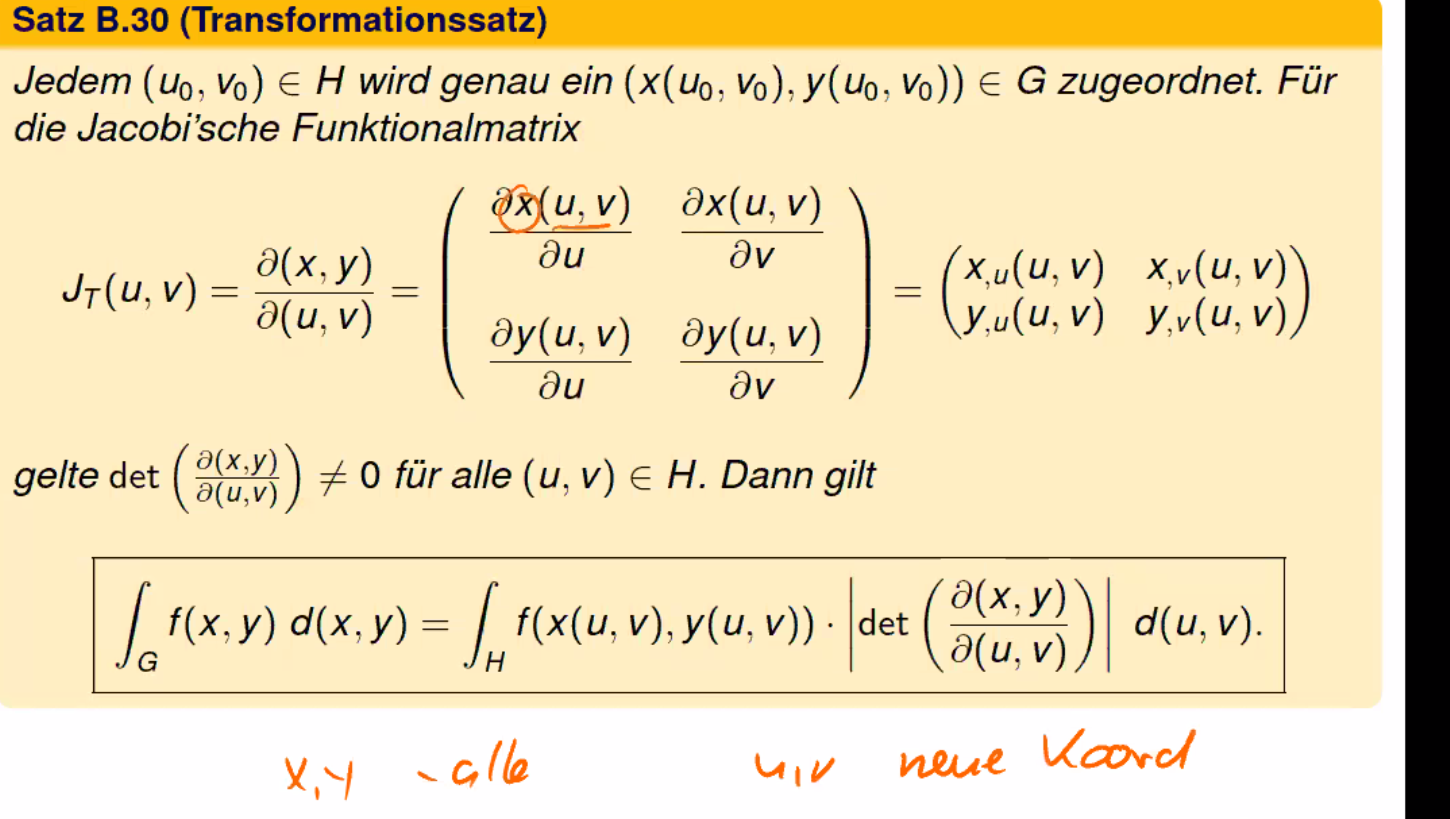
\includegraphics[width=256px]{transformationssatz.png}\\
\end{document}